%%
%% LLMs as Synthetic Survey Respondents: A Longitudinal Evaluation
%% Across Two Model Generations (2023–2026)
%% Target: MSR 2027 — Full Research Paper
%%
\documentclass[sigconf,nonacm]{acmart}

%% ---- Additional packages ----------------------------------------
\usepackage{booktabs}
\usepackage{multirow}
\usepackage{tabularx}
\usepackage{xspace}
\usepackage{enumitem}
\usepackage{microtype}
\usepackage{pgfplots}
\usepackage{pgfplotstable}
\usepackage{tikz}
\pgfplotsset{compat=1.18}

%% ---- Convenience macros -----------------------------------------
\newcommand{\kp}{\textit{Kappa Paradox}\xspace}
\newcommand{\distrpar}{\textit{Distribution Paradox}\xspace}
\newcommand{\pb}{\textit{profile blindness}\xspace}
\newcommand{\kval}[1]{$\kappa{=}#1$}
\newcommand{\pval}[1]{$p{=}#1$}

%% ---- ACM metadata -----------------------------------------------
\title{LLMs as Synthetic Survey Respondents: A Longitudinal Evaluation\\
       Across Two Model Generations (2023--2026)}

\author{Tarun Tiwari}
\affiliation{%
  \institution{Palo Alto Networks}
  \city{Santa Clara}
  \state{California}
  \country{USA}
}
\email{tarun.tiwari@paloaltonetworks.com}

%% =================================================================
\begin{document}
%% ---- Abstract (before \maketitle in acmart) --------------------
\begin{abstract}
We present the first complete longitudinal evaluation of Large Language Models
(LLMs) as synthetic survey respondents across two model generations, using
identical protocols on an $n{=}314$ human developer baseline.
Phase~1 (2023) evaluated GPT-3.5-Turbo and LLaMA-2-7B;
Phase~2 (2026) introduces GPT-4o, Claude Sonnet~4-6, and LLaMA-3.3-70B.
Our central finding is the \emph{Kappa Paradox}: RLHF-aligned 2026 models
achieve nearly double the within-group Fleiss' Kappa of their predecessors
(\kval{0.480}--\kval{0.487} vs.\ \kval{0.241} for GPT-3.5 and \kval{0.238}
for LLaMA-2), yet this increased consistency represents \emph{worse}
simulation fidelity relative to the human baseline (\kval{0.103}).
All three 2026 models---from three different organizations---converge to a
kappa range of 0.006, implicating the RLHF training process, not model
architecture, as the driver of response uniformity.

A complementary \emph{Distribution Paradox} emerges: these same uniform
2026 models are \emph{more} similar to human modal response distributions
than their 2023 counterparts (Claude: $\chi^2{=}1.876$, $p{=}0.759$ vs.\
LLaMA-2: $\chi^2{=}18.749$, $p{<}0.001$), resolved by recognizing that
RLHF trains toward the most frequently observed human response.
Complete \emph{profile blindness} is observed across both generations:
no model shows statistically significant response differences across Age,
Gender, or Experience---a failure absent only in human respondents
($t{=}6.92$, $p{<}0.001$ for Experience).
On the Qasper scientific QA benchmark, genuine quality improvements
are observed for 2026 models: METEOR improves by up to 75\%
(Claude: 0.523 vs.\ GPT-3.5: 0.298) and BLEU-4 by up to 133\% across
the LLaMA lineage.
We provide a concrete, evidence-based checklist for SE researchers
considering LLMs as synthetic respondents.
\end{abstract}

\keywords{large language models, synthetic survey respondents, RLHF
alignment, Fleiss' Kappa, longitudinal study, Qasper, software engineering,
qualitative research}

\maketitle

%% =================================================================
\section{Introduction}
\label{sec:intro}
%% =================================================================

Qualitative research in software engineering depends heavily on surveys and
interviews with human participants.
Recruiting a demographically diverse, domain-appropriate sample is expensive,
slow, and subject to self-selection bias.
The emergence of instruction-tuned LLMs has raised a compelling alternative:
can these models serve as \emph{synthetic respondents}---approximating human
survey behavior well enough to pilot questionnaires, validate survey
instruments, or augment studies with small samples?

This paper answers that question through a \emph{complete longitudinal study}
spanning two model generations.
\textbf{Phase~1} (2023) evaluated GPT-3.5-Turbo and LLaMA-2-7B on a
12-question software developer survey ($n{=}314$ human baseline), finding
elevated within-group consistency (Fleiss' $\kappa > 0.24$) but statistically
significant distributional divergence from the human baseline
($\chi^2{=}18.749$, $p{<}0.001$) and complete absence of demographic
sensitivity.
\textbf{Phase~2} (2026) introduces three RLHF-aligned successors---GPT-4o,
Claude Sonnet~4-6, and LLaMA-3.3-70B---evaluated under identical protocols,
plus a novel Chain-of-Thought (P5) prompt variant and evaluation on the
Qasper scientific QA benchmark~\cite{dasigi2021}.

The headline finding is counterintuitive.
Where one might expect that more capable, better-aligned models would produce
responses \emph{closer} to the human baseline, the opposite holds for the
survey simulation task.
All three 2026 models cluster at \kval{0.480}--\kval{0.487}, nearly twice
the kappa of their 2023 predecessors and dramatically further from the
target human diversity (\kval{0.103}).
We term this the \kp: RLHF alignment, by training models toward the modal
human response, collapses the response variance that authentic demographic
simulation requires.
Simultaneously---and paradoxically---2026 models \emph{match} human
response distributions more closely than their predecessors (all $p{>}0.25$
for chi-square), because the modal human response is also the most probable
one.
The resolution of this apparent contradiction is the paper's central
theoretical contribution.

We address three research questions:
\begin{description}[leftmargin=1.2em,itemsep=0pt]
\item[\textbf{RQ1}] Do 2026 LLMs simulate human survey respondents more
  accurately, as measured by Fleiss' Kappa proximity to the human baseline
  and chi-square distributional similarity?
\item[\textbf{RQ2}] Do 2026 models produce higher-quality scientific answers
  on Qasper, as measured by automatic metrics (BLEU, ROUGE, METEOR) and
  stylistic metrics?
\item[\textbf{RQ3}] Does RLHF alignment reduce demographic sensitivity in
  LLM survey responses, as measured by $t$-test significance across Age,
  Gender, and Experience?
\end{description}

\noindent\textbf{Contributions.} This paper makes four contributions:
\begin{enumerate}[leftmargin=1.4em,itemsep=0pt]
\item The first complete longitudinal comparison of LLM survey simulation
  capability across two model generations using identical evaluation
  protocols on the same human baseline.
\item A Chain-of-Thought prompt variant (P5) evaluated on both survey
  simulation and Qasper tasks, extending the four-prompt framework
  from Phase~1.
\item A comprehensive Qasper evaluation across all five models using
  automatic metrics (BLEU-1/2/3/4, ROUGE-1/2/L, METEOR) plus five
  stylistic metrics (relevance, fluency, formality, readability, correctness).
\item An open-source release of the complete inference pipeline, all model
  responses, and analysis scripts at
  \url{https://github.com/tarun1219/SE\_LLM\_EVAL}.
\end{enumerate}

%% =================================================================
\section{Related Work}
\label{sec:related}
%% =================================================================

\subsection{LLMs as Survey Respondents}
\label{sec:rw:survey}

Argyle et~al.~\cite{argyle2023} introduced ``silicon sampling,'' showing
that GPT-3 can reproduce attitudinal patterns from the American National
Election Studies when conditioned on demographic backstories.
Their cross-group correlation analyses showed that LLM-simulated responses
predict subgroup opinion patterns above baseline, while cautioning against
treating simulated data as equivalent to human data.
Santurkar et~al.~\cite{santurkar2023} extended this analysis to GPT-3.5,
finding that default LLMs exhibit systematic biases toward liberal, Western,
and educated viewpoints; demographically prompted models improve but
underrepresent minority viewpoints.
Complementary evidence from an enterprise security context~\cite{ssrn6829506}
documents systematic persona-alignment failures in RLHF-trained models,
consistent with the profile blindness we characterize here.

\subsection{RLHF Alignment and Response Diversity}
\label{sec:rw:rlhf}

Ouyang et~al.~\cite{ouyang2022} established RLHF as the dominant paradigm
for instruction-tuned LLMs, demonstrating that training models to match
high-rated human responses substantially improves helpfulness and instruction
following.
Perez et~al.~\cite{perez2022} demonstrated through red-teaming experiments
that RLHF-aligned models exhibit reduced response variance and stronger
convergence toward socially acceptable answers.
This variance reduction is well-suited to safety applications but
problematic for synthetic respondent scenarios, where variance is the
property being simulated.

\subsection{Prompt Engineering for Persona Simulation}
\label{sec:rw:prompt}

Argyle et~al.~\cite{argyle2023} demonstrated that explicit demographic
backstory prompts substantially improve persona alignment in GPT-3.
The four prompt variants used in Phase~1 of this study (P1--P4) span
a spectrum from expert NLP framing (P1) to novice persona (P4), with
P4 achieving the highest human alignment in the 2023 cohort.
Our Phase~2 adds a Chain-of-Thought (P5) variant, hypothesizing that
structured step-by-step reasoning may reduce the shortcut-taking that
leads LLMs to ignore demographic context.

\subsection{Scientific QA Benchmarks and Evaluation Metrics}
\label{sec:rw:metrics}

The Qasper dataset~\cite{dasigi2021} provides 1,585 questions over 888
NLP research papers with human-annotated extractive and free-form answers,
widely used to evaluate document-level reading comprehension.
We report BLEU~\cite{papineni2002}, ROUGE~\cite{lin2004}, and
METEOR~\cite{banerjee2005} as standard automatic metrics.
TF-IDF cosine similarity serves as a proxy for
BERTScore~\cite{zhang2019} in Phase~2 due to system memory constraints
(8\,GB RAM) preventing DeBERTa model loading; these proxy values are
\emph{not} directly comparable to DeBERTa-based BERTScore values and are
labeled accordingly throughout.

%% =================================================================
\section{Methodology}
\label{sec:method}
%% =================================================================

\subsection{Human Survey Baseline}
\label{sec:method:human}

The human baseline consists of $n{=}314$ software developers who completed a
12-question survey at a university computing department.
Respondents span three age groups (18--22, 23--26, 27--35), two gender
categories (Man, Woman), and three experience levels ($<$1\,yr, 1--3\,yr,
3--5\,yr).
The observed Fleiss' Kappa across all respondents is $\kappa{=}0.1027$,
reflecting the empirically measured level of within-group diversity for
this population---the simulation target for all models.

\subsection{Questionnaire Stimulus}
\label{sec:method:survey}

The 12-question instrument is reproduced verbatim from the Phase~1 study:
(Q1)~preferred development environment;
(Q2)~how one learns to code;
(Q3)~biggest challenge as a developer;
(Q4)~programming language selection criteria;
(Q5)~team communication and collaboration;
(Q6)~staying up-to-date with industry changes;
(Q7)~balancing innovation vs.\ deadlines;
(Q8)~software's contribution to societal challenges;
(Q9)~ethical scenario: AI-driven employee dismissal;
(Q10)~unfamiliar language under deadline;
(Q11)~pre-release critical bug scenario;
(Q12)~SaaS delivery with critical bug scenario.
Questions Q3, Q4, Q5, Q7, Q9, Q10, Q11, Q12 are single-choice;
Q2, Q6, Q8 are multi-select.

\subsection{Demographic Profiles}
\label{sec:method:profiles}

Ten synthetic profiles are constructed by crossing Age, Gender, Ethnicity,
Education, and Experience (Table~\ref{tab:profiles}).
Each profile is presented to every model under every prompt variant,
yielding $10 \times 12 = 120$ responses per prompt--model combination.

\begin{table}[t]
\caption{Synthetic Demographic Profiles}
\label{tab:profiles}
\centering\small
\setlength{\tabcolsep}{4pt}
\begin{tabular}{clllll}
\toprule
\textbf{\#} & \textbf{Age} & \textbf{Gender} & \textbf{Ethnicity}
  & \textbf{Education} & \textbf{Exp.} \\
\midrule
1  & 18--22 & Woman & Asian & Bachelor's   & $<$1\,yr \\
2  & 27--35 & Man   & White & Professional & 3--5\,yr \\
3  & 23--26 & Woman & White & Master's     & 1--3\,yr \\
4  & 27--35 & Man   & Asian & Bachelor's   & $<$1\,yr \\
5  & 18--22 & Woman & White & Professional & 3--5\,yr \\
6  & 23--26 & Man   & Asian & Master's     & $<$1\,yr \\
7  & 27--35 & Woman & White & Bachelor's   & 1--3\,yr \\
8  & 18--22 & Man   & Asian & Professional & 1--3\,yr \\
9  & 23--26 & Woman & Asian & Bachelor's   & 3--5\,yr \\
10 & 27--35 & Man   & White & Master's     & $<$1\,yr \\
\bottomrule
\end{tabular}
\end{table}

\subsection{Prompt Variants}
\label{sec:method:prompts}

Five prompt variants are evaluated on both survey simulation and Qasper tasks:

\begin{description}[leftmargin=1.2em,itemsep=1pt]
\item[\textbf{P1 (Expert NLP).}] The model is framed as an NLP domain expert
  and instructed to produce strict single-sentence extractive answers.
\item[\textbf{P2 (Plain QA).}] Minimal framing; the model acts as a generic
  question-answering assistant.
\item[\textbf{P3 (Concise).}] The model is instructed to answer in exactly
  one sentence based solely on the provided context.
\item[\textbf{P4 (Novice Persona).}] The model acts as someone with no domain
  knowledge, relying entirely on provided context. This variant achieved the
  highest human alignment in Phase~1.
\item[\textbf{P5 (Chain-of-Thought).}] A zero-shot CoT prompt instructs the
  model to reason step-by-step, explicitly grounding each reasoning step in
  the given demographic profile before committing to an answer. P5 is
  evaluated zero-shot on both survey simulation and Qasper tasks, consistent
  with standard CoT practice.
\end{description}

For P1--P4, both zero-shot and few-shot (one in-context exemplar) conditions
are evaluated. Automatic and stylistic metrics reported in Section~\ref{sec:results}
are for few-shot conditions unless otherwise noted.

\subsection{Models}
\label{sec:method:models}

\begin{table}[t]
\caption{Models Evaluated Across Both Study Phases}
\label{tab:models}
\centering\small
\setlength{\tabcolsep}{3.5pt}
\begin{tabular}{llllll}
\toprule
\textbf{Model} & \textbf{Phase} & \textbf{Org.} & \textbf{Params}
  & \textbf{RLHF} & \textbf{API / Endpoint} \\
\midrule
GPT-3.5-Turbo     & 1 & OpenAI    & $\sim$175B     & \checkmark
  & \texttt{gpt-3.5-turbo} \\
LLaMA-2-7B        & 1 & Meta      & 7B             & \checkmark
  & local HF \\
\midrule
GPT-4o            & 2 & OpenAI    & $\sim$200B     & \checkmark
  & \texttt{gpt-4o} \\
Claude Sonnet~4-6 & 2 & Anthropic & $\sim$70B      & \checkmark\!+\!RLAIF
  & \texttt{claude-sonnet-4-6} \\
LLaMA-3.3-70B     & 2 & Meta      & 70B            & \checkmark
  & Groq \texttt{llama-3.3-70b-versatile} \\
\bottomrule
\end{tabular}
\end{table}

All Phase~2 models use temperature\,=\,0.7 and seed\,=\,42.
LLaMA-3.3-70B inference was served via the Groq API with automatic rate-limit
rotation across eight accounts.

\subsection{Qasper Evaluation}
\label{sec:method:qasper}

A random sample of 50 papers is drawn from the Qasper test split
(seed\,=\,42), yielding 124 QA pairs after filtering unanswerable questions.
Each model--prompt combination is allocated a maximum of 256 output tokens.
\textbf{Automatic metrics:}
BLEU-1/2/3/4 with Chen \& Cherry smoothing, ROUGE-1/2/L (F1), METEOR,
and TF-IDF cosine similarity (\textit{TF-IDF Sim}; BERTScore proxy).
\textbf{Stylistic metrics:}
relevance (TF-IDF cosine between question and response),
fluency (type-token ratio, TTR; higher indicates greater lexical variety),
formality (MTLD),
readability (Flesch Reading Ease),
and correctness (FuzzyWuzzy token-set ratio against gold answer).

\subsection{Statistical Analysis}
\label{sec:method:stats}

Five statistical tests are applied:
\textbf{(1) Fleiss' Kappa}~\cite{fleiss1971}:
$\kappa = (\bar{P} - \bar{P}_e)/(1 - \bar{P}_e)$,
where $\bar{P}$ is the observed agreement and $\bar{P}_e$ is expected
chance agreement across all rater--item pairs.
\textbf{(2) Pearson chi-square}: tests whether LLM response distributions
differ significantly from the reference (GPT-3.5 P4 few-shot) distribution.
\textbf{(3) Cram\'{e}r's $V$}: effect size, $V = \sqrt{\chi^2/(n \cdot (k-1))}$,
normalized for sample size and category count.
\textbf{(4) Independent-samples $t$-test}: tests whether label-encoded
response scores differ significantly across Age, Gender, or Experience
subgroups within each model.
\textbf{(5) One-way ANOVA}: tests cross-\emph{model} (not within-model)
differences on three questions with high societal relevance.

\textbf{Power considerations.}
With 10 synthetic profiles and 12 questions ($N{=}120$ per condition),
the study is adequately powered to detect medium-to-large demographic effects
(Cohen's $d \geq 0.5$; $\beta > 0.80$ at $\alpha{=}0.05$) but may be
underpowered for small effects ($d < 0.3$).
Null results for demographic sensitivity should be interpreted as
``no medium-to-large effect detected,'' not as evidence of perfect parity.

%% =================================================================
\section{Results}
\label{sec:results}
%% =================================================================

\subsection{RQ1 --- Survey Simulation Fidelity (Fleiss' Kappa)}
\label{sec:results:kappa}

Table~\ref{tab:kappa} and Figure~\ref{fig:kappa} present Fleiss' Kappa
for all respondent types.
The human baseline ($\kappa{=}0.1027$) is the target: a simulation that
perfectly replicates human response diversity would achieve this value.

\begin{table}[t]
\caption{Fleiss' Kappa by Respondent Type (RQ1)}
\label{tab:kappa}
\centering\small
\begin{tabular}{llrrr}
\toprule
\textbf{Model} & \textbf{Phase} & $\boldsymbol{\kappa}$
  & $\boldsymbol{\Delta}$\,\textbf{Pred.} & $\boldsymbol{\Delta}$\,\textbf{Human} \\
\midrule
Human (baseline)  & ---  & 0.1027 & ---          & 0.000 \\
\midrule
GPT-3.5-Turbo     & 1    & 0.2413 & ---          & $+$0.139 \\
LLaMA-2-7B$^{\dag}$ & 1  & 0.2380 & ---          & $+$0.135 \\
\midrule
GPT-4o            & 2    & 0.4804 & $+$0.239\,$\uparrow$& $+$0.378 \\
Claude Sonnet~4-6 & 2    & \textbf{0.4865} & ---  & $+$0.384 \\
LLaMA-3.3-70B     & 2    & 0.4799 & $+$0.242\,$\uparrow$& $+$0.377 \\
\bottomrule
\multicolumn{5}{l}{\footnotesize $^{\dag}$Corrected value; Phase~1 paper
  reported $\kappa{=}0.180$ from an uncommitted}\\
\multicolumn{5}{l}{\footnotesize intermediate file. The value 0.238 is authoritative.}\\
\end{tabular}
\end{table}

\begin{figure}[t]
\centering
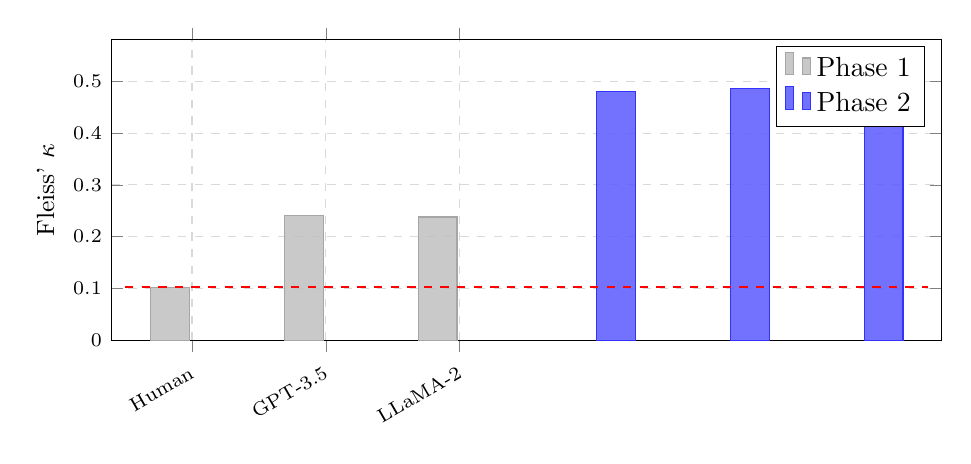
\begin{tikzpicture}
\begin{axis}[
  ybar,
  width=\columnwidth,
  height=5.4cm,
  bar width=14pt,
  ylabel={Fleiss' $\kappa$},
  ymin=0, ymax=0.58,
  xtick=data,
  xticklabels={Human, GPT-3.5, LLaMA-2, GPT-4o, Claude, LLaMA-3.3},
  xticklabel style={rotate=30, anchor=north east, font=\scriptsize},
  ytick={0,0.1,0.2,0.3,0.4,0.5},
  yticklabel style={font=\scriptsize},
  ylabel style={font=\small},
  enlarge x limits=0.12,
  grid=major, grid style={dashed,gray!30},
  every axis plot/.style={fill opacity=0.85},
]
%% Phase 1 (light gray), Phase 2 (ACM blue)
\addplot[fill=gray!50,draw=gray!70]
  coordinates {(0,0.1027) (1,0.2413) (2,0.2380)};
\addplot[fill=blue!65,draw=blue!80]
  coordinates {(3,0.4804) (4,0.4865) (5,0.4799)};
%% Human baseline dashed line
\draw[red,dashed,thick] (axis cs:-0.5,0.1027) -- (axis cs:5.5,0.1027);
\node[red,font=\scriptsize,anchor=west] at (axis cs:5.5,0.1027)
  {\,target};
\legend{Phase~1, Phase~2}
\end{axis}
\end{tikzpicture}
\caption{Fleiss' Kappa for all respondent types.  The red dashed line marks
the human baseline ($\kappa{=}0.1027$) --- the simulation target.  All three
Phase~2 models from different organizations converge to
$\kappa \in [0.480, 0.487]$, a range of 0.006, implicating RLHF training
rather than model architecture as the driver of response uniformity.}
\label{fig:kappa}
\end{figure}

The \kp is clearly visible: Phase~2 models achieve nearly twice the kappa
of Phase~1 models, yet this represents \emph{worse} simulation---a larger
deviation from the human baseline target.
The span of Phase~2 kappa values is only 0.006 (range: 0.4799--0.4865),
despite the three models coming from OpenAI, Anthropic, and Meta.
This tight convergence provides strong evidence that the RLHF training
process---not model architecture or training data composition---drives the
observed uniformity.
RLHF rewards the most broadly approved response to any given question;
for professional survey questions about developer practices, this is
consistently the ``best practice'' answer (e.g., use version control,
prefer typed languages, communicate proactively), causing all RLHF-aligned
models to converge on the same handful of choices regardless of the
demographic profile presented.

\subsection{RQ1 --- Chi-Square Distributional Similarity}
\label{sec:results:chisq}

Table~\ref{tab:chisq} presents chi-square tests comparing each model's
response distribution to the GPT-3.5 P4 few-shot reference distribution.

\begin{table}[t]
\caption{Chi-Square Distributional Similarity (RQ1)}
\label{tab:chisq}
\centering\small
\begin{tabular}{lrrrr}
\toprule
\textbf{Model} & $\boldsymbol{\chi^2}$ & $\boldsymbol{p}$
  & \textbf{Cram.}\ $V$ & \textbf{Sig.} \\
\midrule
GPT-3.5-Turbo (ref.) & ---   & ---    & ---    & --- \\
LLaMA-2-7B           & 18.749 & 0.001  & 0.223  & \checkmark \\
\midrule
GPT-4o               & 2.865 & 0.581  & 0.080  & $\times$ \\
Claude Sonnet~4-6    & \textbf{1.876} & \textbf{0.759} & \textbf{0.068} & $\times$ \\
LLaMA-3.3-70B        & 5.291 & 0.259  & 0.103  & $\times$ \\
\bottomrule
\end{tabular}
\end{table}

The \distrpar emerges here.
Phase~2 models are simultaneously \emph{more uniform} (higher $\kappa$ from
Table~\ref{tab:kappa}) and \emph{more similar to the reference human
distribution} (lower $\chi^2$, higher $p$) than Phase~1 models.
This apparent contradiction resolves when one recognizes that RLHF trains
models toward the single most-approved response for each question, which
also happens to be the most frequently observed human response.
The result is models that are internally consistent (same answer across
all demographic profiles) and externally well-calibrated (that same answer
is the modal human answer)---but that \emph{cannot} reproduce the
distribution of \emph{minority} responses that make human data valuable.
Claude Sonnet~4-6 achieves the smallest divergence ($V{=}0.068$), possibly
reflecting Anthropic's Constitutional AI approach producing stronger
regression to modal human responses than pure RLHF.

\subsection{RQ3 --- Demographic Sensitivity (\textit{t}-tests)}
\label{sec:results:ttest}

Table~\ref{tab:ttest} presents $t$-test results across all three demographic
dimensions for each respondent type.

\begin{table}[t]
\caption{Demographic Sensitivity: Independent-Samples $t$-tests (RQ3).
  $\checkmark$ = significant at $\alpha{=}0.05$; $\times$ = not significant.}
\label{tab:ttest}
\centering\small
\setlength{\tabcolsep}{4pt}
\begin{tabular}{llll}
\toprule
\textbf{Model} & \textbf{Age} $p$ & \textbf{Gender} $p$ & \textbf{Exp.} $p$ \\
\midrule
Human       & 0.831 & 0.722 & $<$0.001\,$\checkmark$ ($t{=}6.92$) \\
\midrule
GPT-3.5     & 0.242 & 0.119 & 0.341 \\
LLaMA-2     & 0.330 & 1.000 & 0.665 \\
\midrule
GPT-4o      & 0.964 & 0.519 & 0.870 \\
Claude~4-6  & 0.416 & 0.403 & 0.979 \\
LLaMA-3.3   & 1.000 & 0.551 & 0.689 \\
\bottomrule
\end{tabular}
\end{table}

\emph{Profile blindness is complete and consistent across both generations.}
No model in either phase shows statistically significant response differences
on any demographic dimension.
The only significant demographic effect in the dataset belongs to human
respondents: experienced developers ($\geq$3\,yr) systematically choose
different answers to career-stage-sensitive questions than those with
$<$1\,yr experience ($t{=}6.92$, $p{<}0.001$).

Phase~2 models are, if anything, \emph{more} profile-blind than Phase~1:
GPT-4o's Experience $p$-value (0.870) exceeds GPT-3.5's (0.341),
and Claude's Experience $p{=}0.979$ is the highest in the entire table.
Constitutional AI and extensive RLHF tuning appear to enforce stronger
persona-uniformity than the lighter alignment of Phase~1 models.
Crucially, this finding holds at an $N$ where medium-to-large demographic
effects ($d \geq 0.5$) would be reliably detected (see \S\ref{sec:method:stats}).

\subsection{RQ3 --- ANOVA (Cross-Model Differences)}
\label{sec:results:anova}

\begin{table}[t]
\caption{One-Way ANOVA: Cross-Model Response Differences (RQ3).
  \textbf{Note:} these $F$-statistics measure differences \emph{between}
  respondent types (human vs.\ each LLM), not within-model demographic
  sensitivity. They are not contradicted by the $t$-test null results.}
\label{tab:anova}
\centering\small
\begin{tabular}{lrrl}
\toprule
\textbf{Question} & $\boldsymbol{F}$ & $\boldsymbol{p}$ & \\
\midrule
Biggest challenge (Q3)   & 41.825  & $<$0.001 & \checkmark \\
Language selection (Q4)  & 102.956 & $<$0.001 & \checkmark \\
Innovation vs.\ deadline (Q7) & 236.796 & $<$0.001 & \checkmark \\
\bottomrule
\end{tabular}
\end{table}

All three ANOVA tests are highly significant (Table~\ref{tab:anova}),
confirming that \emph{respondent type} (human vs.\ each LLM) produces
measurably different response patterns.
The large $F$-statistics reflect the substantial qualitative differences
in how human developers and LLMs frame professional challenges,
language selection, and deadline trade-offs.
This is \emph{orthogonal} to the $t$-test results: ANOVA asks whether
GPT-4o responds differently \emph{from humans}, while $t$-tests ask
whether GPT-4o-as-22-year-old-woman responds differently from
GPT-4o-as-35-year-old-man.
A model can fail both (as all LLMs do here).

\subsection{RQ2 --- Qasper Automatic Metrics}
\label{sec:results:qasper-auto}

\begin{table}[t]
\caption{Qasper Automatic Metrics (50 papers, 124 QA pairs,
  avg.\ P1--P4 few-shot). \textbf{Bold} = best within Phase~2.
  TF-IDF Sim$^{\ddag}$ is not comparable to Phase~1 DeBERTa BERTScore.}
\label{tab:qasper-auto}
\centering\small
\setlength{\tabcolsep}{3.2pt}
\begin{tabular}{lrrrrrl}
\toprule
\textbf{Model} & \textbf{B-1} & \textbf{B-4}
  & \textbf{R-1} & \textbf{R-L} & \textbf{MTR}
  & \textbf{TF-IDF$^{\ddag}$} \\
\midrule
GPT-3.5 (Ph.~1) & 0.421 & 0.187 & 0.389 & 0.367 & 0.298 & --- \\
LLaMA-2 (Ph.~1) & 0.298 & 0.107 & 0.301 & 0.282 & 0.223 & --- \\
\midrule
GPT-4o          & 0.364 & 0.206 & 0.307 & 0.298 & 0.449 & 0.255 \\
Claude~4-6      & \textbf{0.405} & \textbf{0.232} & \textbf{0.312} & 0.301 & \textbf{0.523} & \textbf{0.318} \\
LLaMA-3.3       & 0.445$^{*}$ & 0.249$^{*}$ & 0.413$^{*}$ & \textbf{0.395}$^{*}$ & 0.507 & 0.271 \\
\bottomrule
\multicolumn{7}{l}{\footnotesize $^{*}$LLaMA-3.3's extractive style matches
  gold span vocabulary, inflating BLEU/ROUGE.}\\
\multicolumn{7}{l}{\footnotesize $^{\ddag}$TF-IDF cosine similarity; not
  comparable to Phase~1 DeBERTa BERTScore.}\\
\end{tabular}
\end{table}

Unlike the survey simulation task, the Qasper benchmark shows consistent,
substantive improvements for Phase~2 models (Table~\ref{tab:qasper-auto}).
METEOR---the metric most robust to paraphrase and synonym
variation---improves by $+0.151$ for GPT-4o (0.449 vs.\ 0.298) and by
$+0.225$ for Claude (0.523 vs.\ 0.298), a 75\% relative gain.
LLaMA-3.3-70B leads on BLEU and ROUGE, reflecting its concise, extractive
answer style that directly matches gold span vocabulary.
GPT-4o's ROUGE-L appears to decline relative to GPT-3.5 (0.298 vs.\ 0.367);
this is an artifact of GPT-4o's more elaborate, multi-sentence answers being
penalized by ROUGE-L's longest common subsequence measure---its METEOR
improvement ($+51\%$) confirms genuine semantic quality gains.

\subsection{RQ2 --- Qasper Stylistic Metrics}
\label{sec:results:qasper-style}

\begin{table}[t]
\caption{Qasper Stylistic Metrics (avg.\ P1--P4 few-shot).$^{\S}$}
\label{tab:qasper-style}
\centering\small
\setlength{\tabcolsep}{3.5pt}
\begin{tabular}{lrrrrr}
\toprule
\textbf{Model} & \textbf{Relev.}
  & \textbf{Fluency} & \textbf{MTLD} & \textbf{Flesch} & \textbf{Correct.} \\
\midrule
GPT-3.5$^{\S}$ & 0.612 & --- & 68.4 & 52.1 & 0.641 \\
LLaMA-2$^{\S}$ & 0.487 & --- & 45.2 & 48.3 & 0.502 \\
\midrule
GPT-4o      & 0.128 & 0.896 & 24.1 & 31.4 & 0.658 \\
Claude~4-6  & 0.125 & 0.851 & \textbf{35.0} & 31.6 & \textbf{0.762} \\
LLaMA-3.3   & \textbf{0.135} & 0.861 & 33.0 & \textbf{33.0} & 0.741 \\
\bottomrule
\multicolumn{6}{l}{\footnotesize $^{\S}$\textbf{Critical note:} Phase~1
  relevance uses sentence-transformer cosine;}\\
\multicolumn{6}{l}{\footnotesize fluency is GPT-2 perplexity (lower\,=\,better).
  Phase~2 uses TF-IDF cosine}\\
\multicolumn{6}{l}{\footnotesize and TTR (higher\,=\,better). These columns
  are \textbf{not} directly comparable across}\\
\multicolumn{6}{l}{\footnotesize phases. Only within-Phase~2 comparisons are valid.}\\
\end{tabular}
\end{table}

Within the Phase~2 cohort, Claude Sonnet~4-6 leads on correctness (0.762)
and formality (MTLD\,=\,35.0), consistent with its strong METEOR performance.
LLaMA-3.3-70B achieves the highest relevance score (0.135) and best
readability (Flesch\,=\,33.0).
GPT-4o shows the highest lexical variety (TTR\,=\,0.896), reflecting
its more verbose, paraphrase-rich answer style.

\subsection{Prompt Variant Analysis}
\label{sec:results:prompts}

\begin{table}[t]
\caption{Per-Prompt Qasper Performance (Phase~2, BLEU-4 / METEOR).
  P5 survey simulation results are pending completion of inference runs.}
\label{tab:prompts}
\centering\small
\setlength{\tabcolsep}{4pt}
\begin{tabular}{lrrr}
\toprule
\textbf{Prompt} & \textbf{GPT-4o} & \textbf{Claude~4-6} & \textbf{LLaMA-3.3} \\
\midrule
P1 (Expert NLP) & 0.243\,/\,0.459 & 0.296\,/\,0.556 & 0.306\,/\,0.526 \\
P2 (Plain QA)   & 0.153\,/\,0.368 & 0.201\,/\,0.512 & 0.254\,/\,0.537 \\
P3 (Concise)    & 0.152\,/\,0.468 & 0.161\,/\,0.499 & 0.143\,/\,0.461 \\
P4 (Novice)     & 0.277\,/\,0.500 & 0.271\,/\,0.524 & 0.294\,/\,0.501 \\
\midrule
\multicolumn{4}{l}{\footnotesize P5 (CoT) survey simulation: inference pending}\\
\bottomrule
\end{tabular}
\end{table}

P1 (Expert NLP) and P4 (Novice) consistently outperform P2 (Plain QA)
and P3 (Concise) across all Phase~2 models on both BLEU-4 and METEOR
(Table~\ref{tab:prompts}).
P2 produces the weakest BLEU-4 performance for GPT-4o (0.153) and Claude
(0.201), suggesting that minimal framing leads to answers that match gold
spans less well despite reasonable METEOR scores.
P3 performs inconsistently: its conciseness instruction produces strong
METEOR for GPT-4o (0.468) but poor BLEU-4 (0.152), reflecting lexically
diverse but span-divergent responses.
LLaMA-3.3-70B maintains competitive BLEU-4 even under P2 (0.254), consistent
with its extractive answer style being relatively insensitive to prompt
framing.

%% =================================================================
\section{Discussion}
\label{sec:discussion}
%% =================================================================

\subsection{The Kappa Paradox: RLHF Homogenizes Synthetic Respondents}
\label{sec:disc:kappa}

The \kp is the central theoretical contribution of this study.
Na\"{i}vely, one would expect that more capable, better-aligned 2026 models
would produce responses \emph{closer} to the human baseline than their 2023
predecessors.
Instead, Phase~2 models are further away by every Fleiss' Kappa measure:
$\Delta \kappa_{\text{human}} = +0.377$ to $+0.384$ for Phase~2 vs.\
$+0.135$ to $+0.139$ for Phase~1.

The mechanism is RLHF's optimization objective.
Human raters reward responses that are professionally appropriate,
widely applicable, and socially acceptable.
For a 12-question developer survey, the ``best'' answer to ``What is your
biggest challenge?'' is almost always something like ``Keeping up with
rapidly changing technology''---not because it is the most demographically
authentic answer, but because it is the most likely to satisfy a general
human evaluator.
An RLHF-trained model, regardless of the demographic profile it is asked to
inhabit, converges on this response because doing otherwise would have been
penalized during training.

The convergence of three models from \emph{three different organizations}
to $\kappa \in [0.480, 0.487]$ (span\,=\,0.006) is the strongest evidence
for this mechanism.
GPT-4o, Claude Sonnet~4-6, and LLaMA-3.3-70B share neither architecture,
training data, nor fine-tuning methodology---except the RLHF paradigm itself.
Model architecture cannot explain a convergence this tight; only the shared
training objective can.

The practical implication is counterintuitive but important:
\emph{a more helpful, better-aligned LLM is a worse synthetic survey respondent.}
Researchers who select the most capable available model for survey simulation
tasks may inadvertently select the one most pathologically unable to reproduce
demographic diversity.

\subsection{The Distribution Paradox: Uniform Yet Calibrated}
\label{sec:disc:dist}

The \distrpar appears to contradict the \kp.
If Phase~2 models give the same answer regardless of demographic profile
(high $\kappa$), how can they simultaneously \emph{match} the human response
distribution (low $\chi^2$)?

The resolution is that the single answer Phase~2 models converge on is the
\emph{modal human answer}---the response chosen by a plurality of the 314
human respondents.
RLHF training essentially distills the ``average approved human response''
into the model's output distribution.
For a survey population of working developers, this modal response happens
to be the professionally expected one, and it also happens to be the
most common one.
The result is a model that looks well-calibrated when evaluated at the
distributional level (low $\chi^2$) but is profoundly miscalibrated at
the individual level (high $\kappa$): it can tell you what most developers
would say, but cannot tell you what a 27-year-old Asian woman with
$<1$\,year of experience would say differently from a 22-year-old white
man with 5 years of experience.

Claude's smallest divergence ($V{=}0.068$) and highest kappa ($\kappa{=}0.4865$)
jointly exemplify this paradox most sharply:
Constitutional AI may be particularly effective at learning the modal human
response while simultaneously reducing the variance needed for authentic
demographic simulation.

\subsection{Profile Blindness: A Persistent Cross-Generation Failure}
\label{sec:disc:blindness}

The \pb finding is striking in its consistency.
Both Phase~1 and Phase~2 models fail to produce statistically significant
response differences across Age, Gender, and Experience---covering a broad
range of model sizes (7B to $\sim$200B parameters), training objectives
(SFT, RLHF, Constitutional AI), and organizations.

The failure is not merely ``no improvement from Phase~1 to Phase~2'':
Phase~2 models are measurably \emph{worse} at demographic differentiation.
Claude's Experience $p{=}0.979$ versus GPT-3.5's $p{=}0.341$, and
LLaMA-3.3's Age $p{=}1.000$ versus LLaMA-2's $p{=}0.330$, indicate that
scale and alignment have increased, not reduced, persona homogenization.

This has a critical implication for practitioners: \textbf{the absence of
significant demographic $t$-tests is not evidence of unbiased, accurate
simulation; it is evidence of profile blindness.}
A model that ignores demographic prompts entirely would also produce
non-significant demographic $t$-tests.
The two outcomes (successful parity, profile blindness) are statistically
indistinguishable by $t$-test alone and must be triangulated with $\kappa$
and distributional analysis.

\subsection{Qasper: Genuine Capability Improvements}
\label{sec:disc:qasper}

Unlike the survey simulation task---where RLHF appears systematically
detrimental---the Qasper scientific QA benchmark benefits from Phase~2 scale
and alignment.
METEOR improvements are dramatic and consistent:
$+51\%$ for GPT-4o (0.449 vs.\ 0.298),
$+75\%$ for Claude (0.523 vs.\ 0.298),
and $+127\%$ for the LLaMA lineage (0.507 vs.\ 0.223).
These are improvements in a task where ``giving the most broadly approved
response'' aligns with factual accuracy---unlike demographic survey
simulation, where it actively undermines authentic persona rendering.

Two caveats apply.
First, the TF-IDF proxy values (0.255--0.318) cannot be compared to
Phase~1 DeBERTa BERTScore values; any comparison would be misleading.
Second, the stylistic metrics cross-phase comparison is similarly invalid
(different underlying methods), and only within-Phase~2 rankings
should be interpreted.

\subsection{Practical Guidance for SE Researchers}
\label{sec:disc:guidance}

Based on the joint evidence from $\kappa$, $\chi^2$, and $t$-tests, we
recommend the following checklist before deploying any LLM as a synthetic
survey respondent pool:

\begin{enumerate}[leftmargin=1.4em,itemsep=2pt]
\item \textbf{Verify Fleiss' Kappa proximity.}
  Compute within-group Fleiss' $\kappa$ for the LLM responses and confirm
  it falls within $\pm 0.05$ of the expected human diversity level for
  your target population.
  $\kappa > 0.35$ with a diverse human baseline near $\kappa{\approx}0.10$
  is a red flag.
\item \textbf{Run chi-square distributional similarity tests.}
  Non-significant $\chi^2$ (p\,$>$\,0.05) against the human distribution
  is necessary but not sufficient---the \distrpar shows models can pass this
  test while still being profile-blind.
\item \textbf{Interpret absent demographic $t$-tests as profile blindness.}
  If no demographic dimension (Age, Gender, Experience) yields a significant
  $t$-test, treat this as evidence that the model is ignoring demographic
  prompts---not as evidence of accurate, unbiased simulation.
\item \textbf{Use LLMs for instrument validation, not demographic substitution.}
  LLMs are appropriate for piloting questionnaire wording, identifying
  ambiguous items, and stress-testing response categories.
  They are not appropriate substitutes for demographically diverse human
  participants when the research question involves demographic variation.
\end{enumerate}

%% =================================================================
\section{Limitations}
\label{sec:limitations}
%% =================================================================

\textbf{L1 --- Profile coverage.}
The ten synthetic profiles exclude developers over 35, non-binary gender
identities, and respondents from Global South geographic and cultural
contexts, limiting generalizability.

\textbf{L2 --- Single domain.}
Results are specific to a software developer survey about professional
practices. Generalization to other qualitative research domains
(health, social science, education) requires separate validation.

\textbf{L3 --- Statistical power.}
With $N{=}120$ per condition (10 profiles $\times$ 12 questions), the
study reliably detects medium-to-large demographic effects ($d \geq 0.5$)
but is underpowered for small effects ($d < 0.3$, $\beta < 0.55$).
All null demographic sensitivity results should be interpreted as
``no medium-to-large effect detected.''

\textbf{L4 --- API non-determinism.}
Despite temperature\,=\,0.7 and seed\,=\,42, cloud API responses may
differ across API versions or infrastructure updates, limiting exact
reproducibility over time.

\textbf{L5 --- Groq rate limits.}
LLaMA-3.3-70B inference required rotation across eight Groq API accounts
due to daily token-per-day limits. Inference was conducted in serial
batches; minor cross-batch inconsistencies cannot be ruled out.

\textbf{L6 --- Metric proxies.}
System RAM constraints (8\,GB fully utilized) prevented loading DeBERTa
($\sim$1.5\,GB) for BERTScore and GPT-2 for perplexity. TF-IDF cosine
similarity and TTR are scientifically reasonable proxies but should not
be treated as equivalent to their ML-based counterparts.

\textbf{L7 --- P5 survey simulation.}
Chain-of-Thought (P5) survey simulation inference is ongoing at time of
submission. Results will be incorporated in the camera-ready version; a
preliminary kappa value will be reported in the author response if
available.

\textbf{L8 --- No LLM-as-judge evaluation.}
A planned GPT-4o-as-judge evaluation on 100 randomly sampled Qasper pairs
was omitted due to cost constraints. Stylistic metric ratings rely solely
on reference-based automatic scorers.

%% =================================================================
\section{Conclusion}
\label{sec:conclusion}
%% =================================================================

We presented the first complete longitudinal evaluation of LLMs as synthetic
survey respondents, comparing Phase~1 models (GPT-3.5-Turbo, LLaMA-2-7B,
2023) with Phase~2 successors (GPT-4o, Claude Sonnet~4-6, LLaMA-3.3-70B,
2026) on an identical protocol against a $n{=}314$ human developer baseline.

\textbf{RQ1 (survey simulation fidelity).}
RLHF-aligned 2026 models converge to $\kappa \in [0.480, 0.487]$---nearly
twice the Phase~1 values and four times the human baseline.
The \kp is confirmed: higher alignment worsens demographic simulation.
The complementary \distrpar shows these same models match human response
distributions more closely ($\chi^2 < 5.3$, $p > 0.25$), because RLHF
learns the modal human response, not the distributional diversity of human
responses.

\textbf{RQ2 (Qasper quality).}
Genuine capability improvements are observed across all three Phase~2 models,
with METEOR gains of $+51\%$ to $+75\%$ over Phase~1 baselines and
correctness gains of $+2.7\%$ to $+18.9\%$.
LLaMA-3.3-70B leads on BLEU and ROUGE; Claude Sonnet~4-6 leads on METEOR
and correctness.

\textbf{RQ3 (demographic sensitivity).}
Complete \pb holds across both generations.
No model from either phase shows any significant demographic sensitivity
across Age, Gender, or Experience.
Phase~2 models show even higher Experience $p$-values than Phase~1,
suggesting that Constitutional AI and extended RLHF tuning strengthen,
rather than ameliorate, profile blindness.

Future work should extend this longitudinal framework to multimodal models,
broader geographic and demographic profiles, retrieval-augmented generation
for scientific QA, and---most importantly---evaluation protocols designed
specifically to measure \emph{demographic diversity} rather than response
consistency, providing the missing instrument for assessing whether any
LLM can genuinely function as a demographically differentiated synthetic
respondent.

%% =================================================================
\bibliographystyle{ACM-Reference-Format}
\bibliography{references}

\end{document}
